\documentclass[crop,class=article]{standalone}
%----------------------------Preamble-------------------------------%
\usepackage{tikz}           % Drawing/graphing tools.
\usetikzlibrary{
    arrows.meta,            % Latex and Stealth arrows.
    decorations.markings    % Adding arrows in the middle of a line.
}
%--------------------------Main Document----------------------------%
\begin{document}
    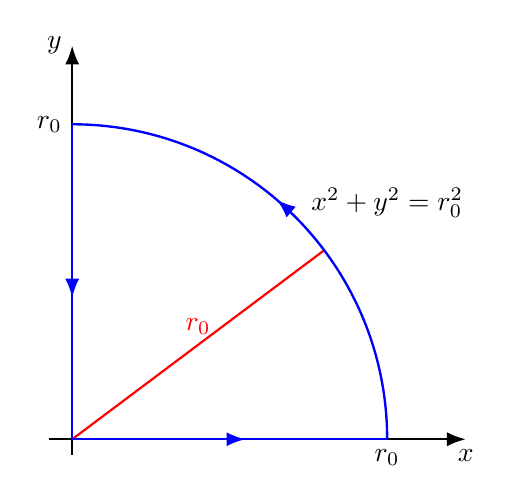
\begin{tikzpicture}[%
        line width=0.3mm,
        >=Latex,
        ->-/.style={
            decoration={
                markings,
                mark=at position .55 with \arrow{>}
            },
            postaction={decorate}
        }
    ]
            \draw[->] (-0.3,0) to (5,0) node [below] {$x$};
            \draw[->] (0,-0.2) to (0,5) node [left] {$y$};
            \draw[red,thick] (0,0) to
                node [above] {$r_{0}$} (3.2,2.4);
            \draw[->-,blue] (0,0) -- (4,0);
            \draw[->-,blue] (0,4) -- (0,0);
            \draw[->-,blue] (4,0) arc (0:90:4);
            \node at (4,3) {$x^2+y^2=r_{0}^{2}$};
            \node at (4,0) [below] {$r_{0}$};
            \node at (0,4) [left] {$r_{0}$};
    \end{tikzpicture}
\end{document}